\clearpage
\makeatletter
\efloat@restorefloats
\makeatother


\begin{appendix}
\section{Recruitment \& data
exclusions}\label{recruitment-data-exclusions}

\begin{figure} [!htb]
\centering
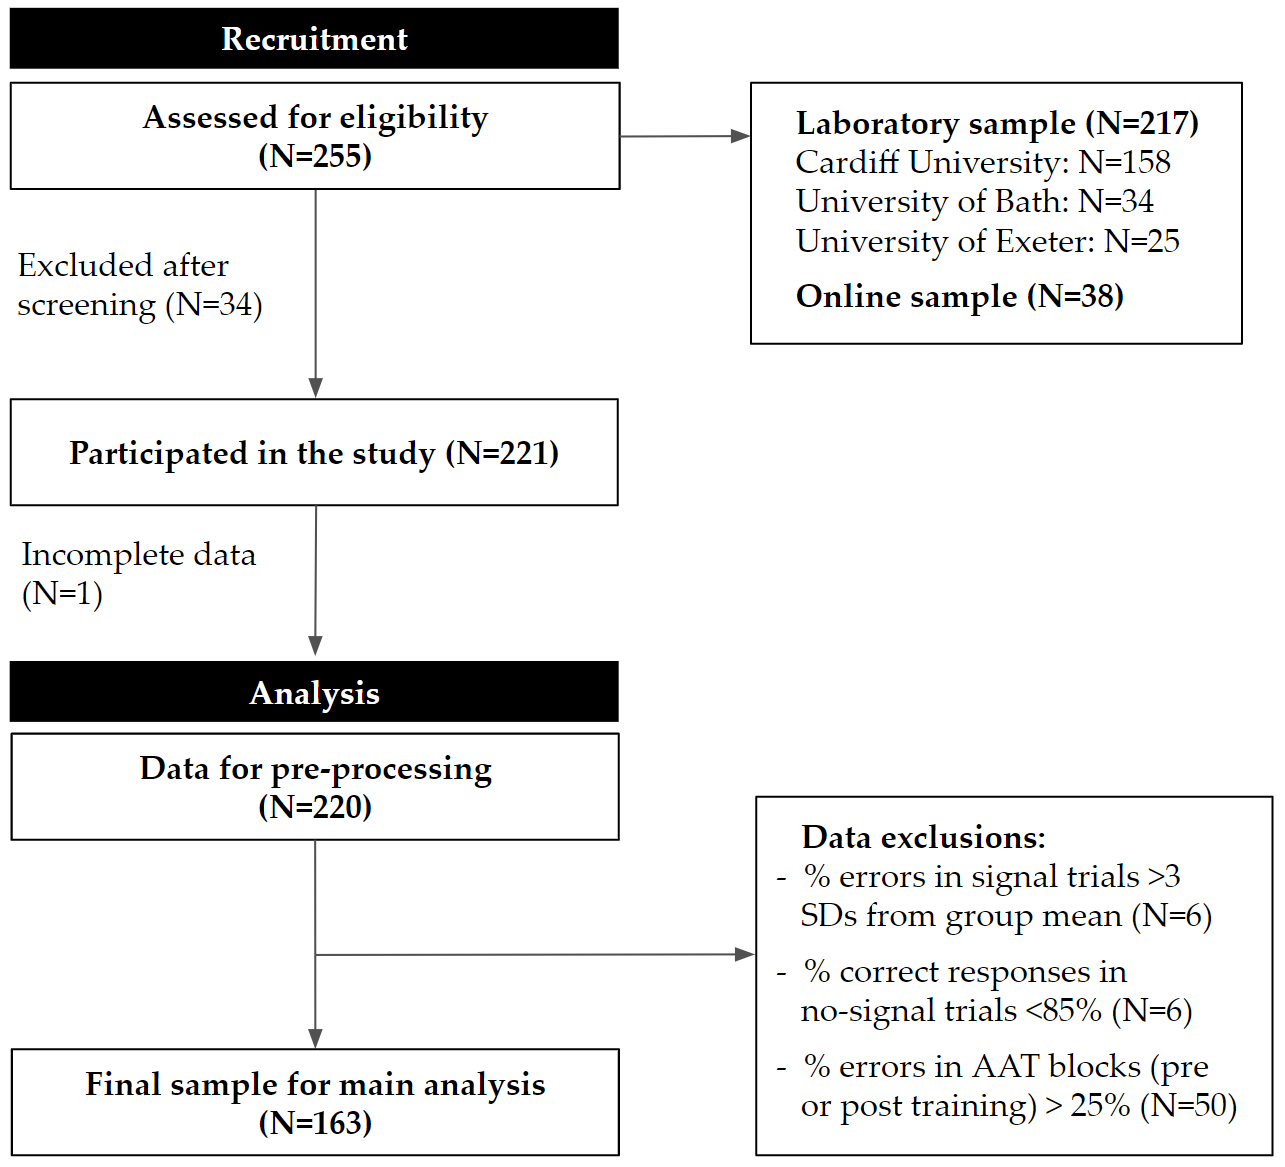
\includegraphics[width=0.7\linewidth]{figures/FigureA1.png}
\captionof{figure}{\textbf{Flow diagram of recruitment and participant-level data exclusions.} There were 255 individuals recruited and assessed for eligibility across laboratory sites and online via personal communication. 34 participants were excluded after screening for not meeting the advertised inclusion/exclusion criteria and we obtained datasets from 221 participants. The online sample was recruited by the University of Bath and University of Exeter. One participant was excluded for providing incomplete data and 220 datasets were submitted for pre-processing and inspection. There we no participants with a mean reaction time on no-sginal trials (GoRT) greater than three standard deviations (SDs) from the group mean and there we no cases of consistently missed (i.e., default option of 50) responses on food rating trials. Six participants had a percentage of errors in signal trials was greater than three SDs from the group mean and six participants also had a percentage of correct responses in no-signal trials lower than 85\%. Please note that some participants met more than one exclusion criterion. 50 participants were excluded as their percentage of errors in either the pre- or post-training approach-avoidance task (AAT) blocks was greater than 25\%. The final sample consisted of 163 participants.}
\label{fig:recruitment}
\end{figure}
\end{appendix}
